\documentclass[11pt,a4paper]{article}

% ── packages ─────────────────────────────────────────────────────────────────
\usepackage[margin=2cm]{geometry}
\usepackage{graphicx}
\usepackage{booktabs}
\usepackage{array}
\usepackage{tabularx}
\usepackage{xcolor}
\usepackage{hyperref}
\usepackage{titlesec}
\usepackage{parskip}
\usepackage{microtype}
\usepackage{caption}
\usepackage{subcaption}
\usepackage{float}
\usepackage{amsmath}
\usepackage{enumitem}
\usepackage{fancyhdr}
\usepackage{mdframed}

% ── colours ──────────────────────────────────────────────────────────────────
\definecolor{lightgray}{RGB}{245,245,245}
\definecolor{darkgray}{RGB}{80,80,80}

% ── hyperlinks — black, no coloured boxes ────────────────────────────────────
\hypersetup{
  colorlinks=true,
  linkcolor=black,
  urlcolor=black,
  citecolor=black,
}

% ── section styling — black ──────────────────────────────────────────────────
\titleformat{\section}{\large\bfseries}{}{0em}{}[\titlerule]
\titleformat{\subsection}{\normalsize\bfseries}{}{0em}{}
\titlespacing*{\section}{0pt}{12pt}{6pt}
\titlespacing*{\subsection}{0pt}{8pt}{4pt}

% ── header / footer ──────────────────────────────────────────────────────────
\pagestyle{fancy}
\fancyhf{}
\renewcommand{\headrulewidth}{0.4pt}
\fancyhead[L]{\small\textcolor{darkgray}{IVADL Assignment 2 --- Skin Disease Object Detection}}
\fancyhead[R]{\small\textcolor{darkgray}{SS 2026}}
\fancyfoot[C]{\small\thepage}

% ── captions: consistent serif font, centred label, proper spacing ────────────
\captionsetup{
  font       = small,
  labelfont  = {bf},
  textfont   = {normalfont},
  skip       = 8pt,
  justification = justified,
  margin     = 0.4cm,
}
\captionsetup[subfigure]{
  font       = footnotesize,
  labelfont  = {bf},
  textfont   = {normalfont},
  skip       = 5pt,
  justification = centering,
  margin     = 0pt,
  position   = below,
}
\captionsetup[table]{
  skip       = 4pt,
  position   = below,
}

% ── image base path ──────────────────────────────────────────────────────────
\graphicspath{{../outputs/plots/}{../outputs/comparison/}{../runs/skin_yolo11n/}}

% ─────────────────────────────────────────────────────────────────────────────
\begin{document}

% ── title block ──────────────────────────────────────────────────────────────
\begin{center}
  {\LARGE\bfseries Assignment 2}\\[6pt]
  {\large Object Detection with YOLO11n on Skin Disease Images}\\[10pt]
  {\normalsize Image and Video Analysis with Deep Learning \quad|\quad SS 2026}\\[6pt]
  {\normalsize
    \textbf{Narseyit Shyngys}\quad
    \textbf{Malikov Fakhri}\quad
    \textbf{Golovatenko Vladislav}
  }\\[4pt]
  {\small May 2026}
\end{center}
\vspace{4pt}
\noindent\rule{\linewidth}{1.5pt}
\vspace{6pt}

% ─────────────────────────────────────────────────────────────────────────────
\section{Dataset}

\textbf{Source:} Roboflow Universe ---
\href{https://universe.roboflow.com/skin-diseases-iyitj/skin-k1hhx/dataset/4}{skin-diseases-iyitj/skin-k1hhx v4}
(License: CC~BY~4.0)

\textbf{Domain:} Clinical and dermoscopic skin lesion photography --- visually distinct from the
80 MS~COCO classes (people, vehicles, household objects) used to pre-train YOLO11n, making it a
meaningful domain-adaptation challenge.

\textbf{Classes (2):} \textbf{Eczema} \quad \textbf{melanoma-disease}

\begin{center}
\begin{tabular}{lccc}
\toprule
\textbf{Split} & \textbf{Train} & \textbf{Validation} & \textbf{Test} \\
\midrule
Images & 145 & 41 & 21 \\
\bottomrule
\end{tabular}
\captionof{table}{Dataset split sizes (207 images total).}
\end{center}

% ─────────────────────────────────────────────────────────────────────────────
\section{Model Selection}

\textbf{Model:} \texttt{YOLO11n} (Ultralytics, nano variant) \quad
\textbf{Pre-trained on:} MS COCO 2017 (80 classes)

\begin{mdframed}[backgroundcolor=lightgray, linecolor=black, linewidth=0.8pt,
                 innertopmargin=7pt, innerbottommargin=7pt,
                 innerleftmargin=10pt, innerrightmargin=10pt]
\textbf{Justification:} YOLO11n ($\approx$2.6\,M parameters, 5.4\,MB weight file) is the
smallest variant of the YOLO11 family. It trains feasibly on consumer hardware using Apple
MPS acceleration within the time budget. Compared to YOLOv8n, YOLO11 features an improved
C2PSA attention block and a redesigned neck, yielding a small mAP gain at the same inference
speed. The nano size ensures batch=16 at 640\,px fits comfortably in memory without
out-of-memory risk.
\end{mdframed}

% ─────────────────────────────────────────────────────────────────────────────
\section{Baseline Results (Pre-trained, No Fine-Tuning)}

The pre-trained YOLO11n was applied to all 21 test images at a confidence threshold of 0.25,
without any adaptation to the skin-disease domain.

Because YOLO11n's 80 COCO classes contain no skin-disease categories, the model produces
\textbf{no valid detections}: it occasionally fires spurious predictions on structurally similar
COCO objects (e.g., textures resembling \emph{sports ball} or \emph{frisbee}) but at very low
confidence. The formal mAP50 for \texttt{melanoma-disease} is exactly 0.000.

\begin{figure}[H]
  \centering
  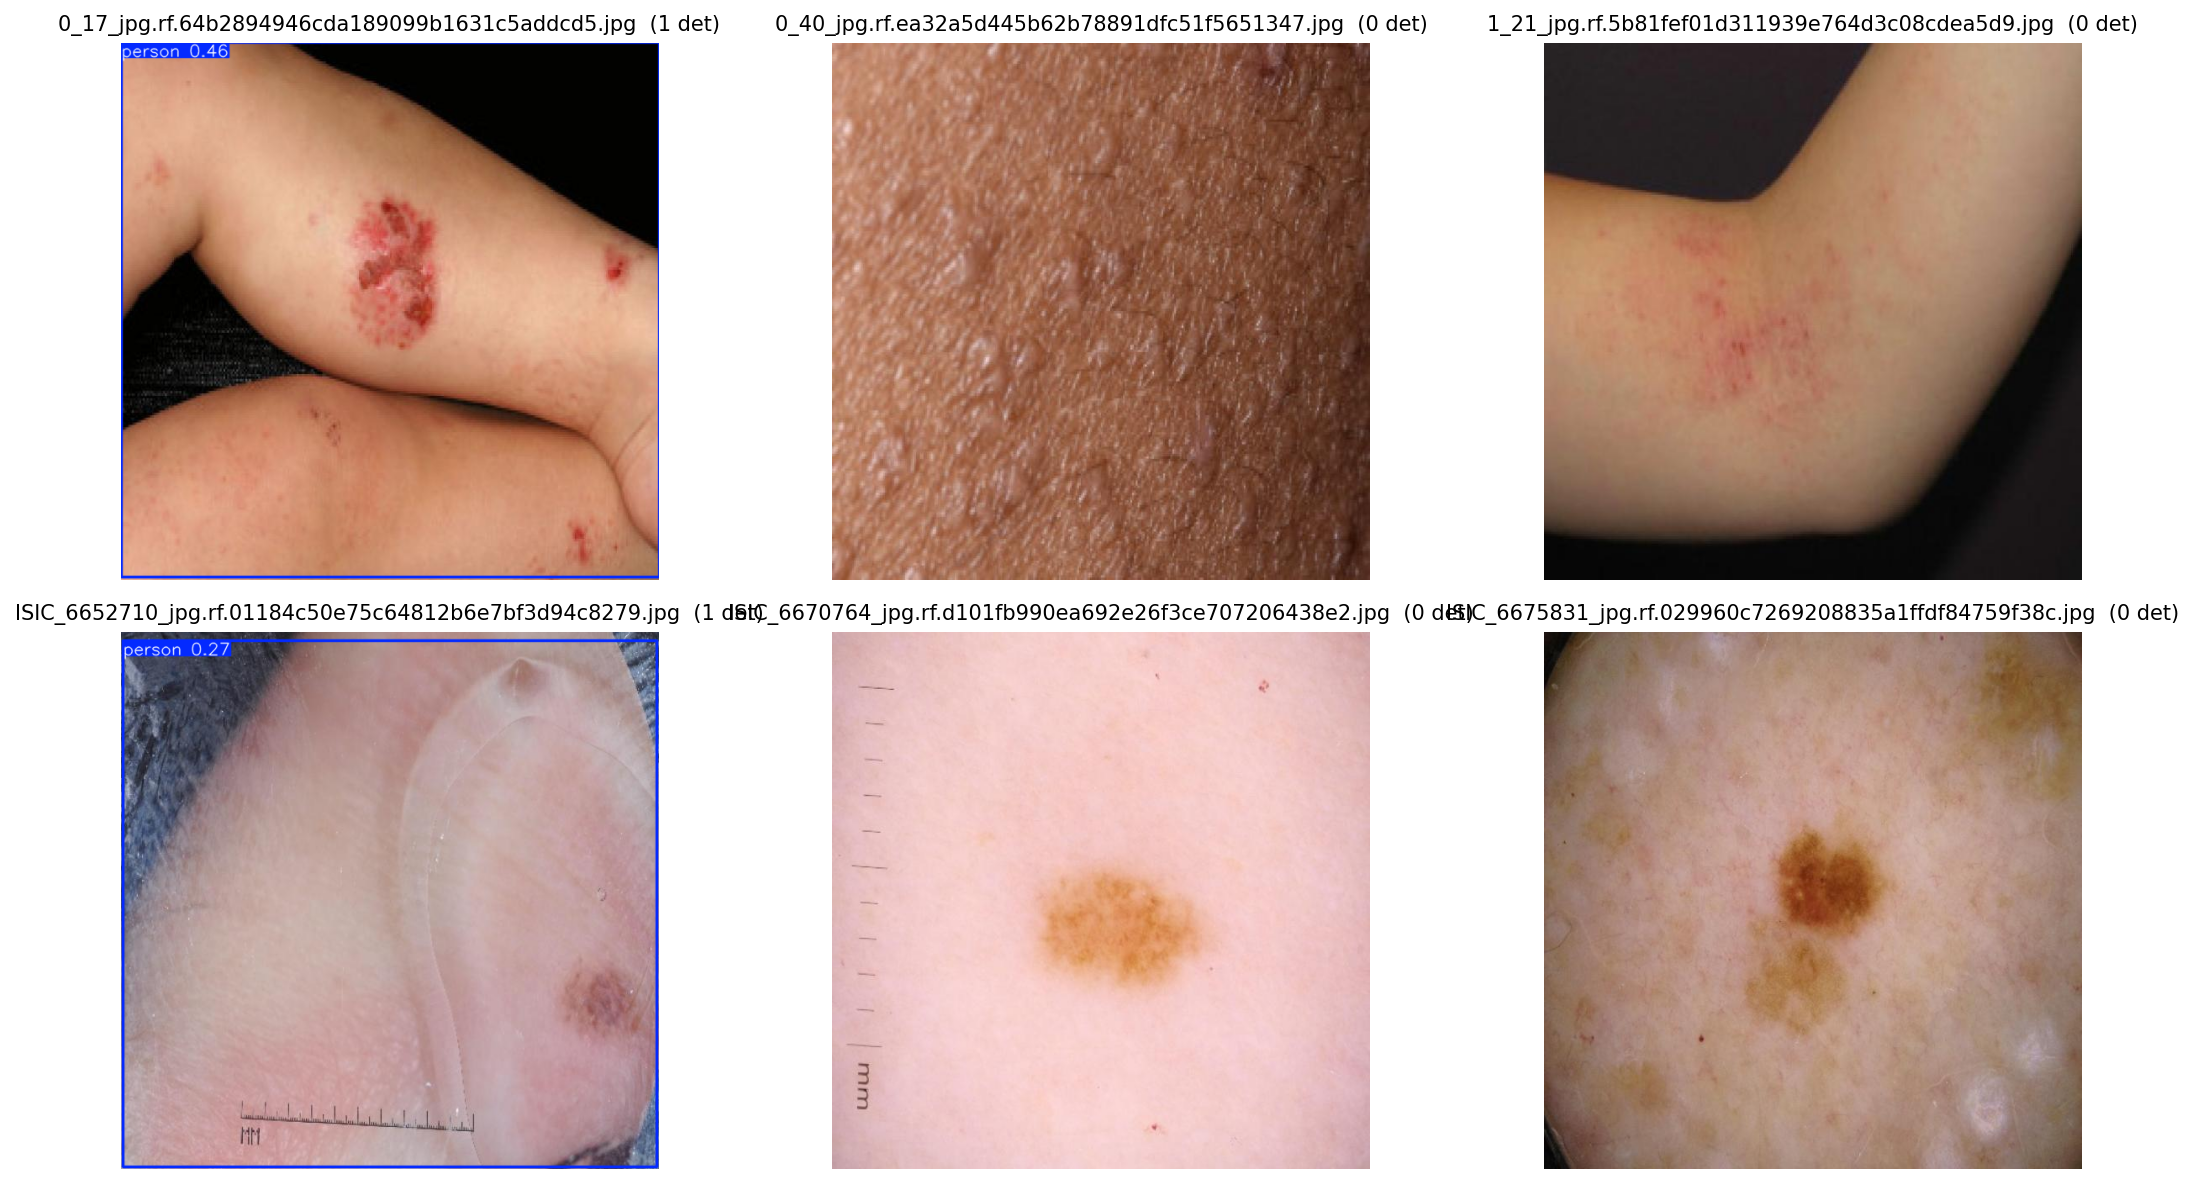
\includegraphics[width=\linewidth]{baseline_grid.png}
  \caption{Baseline predictions on 6 example test images. Most images show zero detections;
           the COCO-pretrained model cannot recognise skin lesions.}
\end{figure}

% ─────────────────────────────────────────────────────────────────────────────
\section{Fine-Tuning Setup}

\begin{center}
\begin{tabular}{ll}
\toprule
\textbf{Parameter} & \textbf{Value} \\
\midrule
Base weights        & \texttt{yolo11n.pt} (COCO pre-trained) \\
Epochs              & 50 (early stop patience = 15) \\
Batch size          & 16 \\
Input resolution    & $640 \times 640$\,px \\
Frozen layers       & None (\texttt{freeze=0}, full fine-tune) \\
Device              & Apple Silicon (MPS) \\
Seed                & 42 \\
Training time       & 11 minutes \\
\bottomrule
\end{tabular}
\captionof{table}{Fine-tuning configuration.}
\end{center}

\textbf{Freeze decision:} All layers were fine-tuned (\texttt{freeze=0}) because the target domain
(dermoscopic skin lesions) is visually far from COCO. Freezing the backbone would retain COCO
features that do not transfer to subtle lesion boundaries. Full fine-tuning allows the entire
network to adapt to the new domain.

\begin{figure}[H]
  \centering
  \includegraphics[width=\linewidth]{results.png}
  \caption{Training curves over 50 epochs. Loss consistently decreases while validation mAP50
           converges to $\approx$0.975 on the validation split.}
\end{figure}

% ─────────────────────────────────────────────────────────────────────────────
\section{Evaluation and Comparison}

Both models were evaluated on the 21-image \textbf{test split} using
\texttt{model.val(split="test")}.

% ── 5.1 Quantitative ────────────────────────────────────────────────────────
\subsection{Quantitative Results}

\begin{center}
\begin{tabular}{lrrrr}
\toprule
\textbf{Metric} & \textbf{Baseline} & \textbf{Fine-tuned} & $\boldsymbol{\Delta}$ \\
\midrule
Precision (overall)               & 0.766 & \textbf{0.901} & +0.135 \\
Recall (overall)                  & 0.229 & \textbf{0.949} & +0.720 \\
mAP50 (overall)                   & 0.260 & \textbf{0.951} & +0.691 \\
mAP50-95 (overall)                & 0.172 & \textbf{0.720} & +0.548 \\
\midrule
mAP50 \textemdash{} Eczema              & 0.520 & \textbf{0.995} & +0.475 \\
mAP50 \textemdash{} melanoma-disease    & 0.000 & \textbf{0.906} & +0.906 \\
\midrule
mAP50-95 \textemdash{} Eczema           & 0.344 & \textbf{0.815} & +0.471 \\
mAP50-95 \textemdash{} melanoma-disease & 0.000 & \textbf{0.625} & +0.625 \\
\bottomrule
\end{tabular}
\captionof{table}{Test-split metrics: baseline vs.\ fine-tuned YOLO11n.}
\end{center}

\begin{figure}[H]
  \centering
  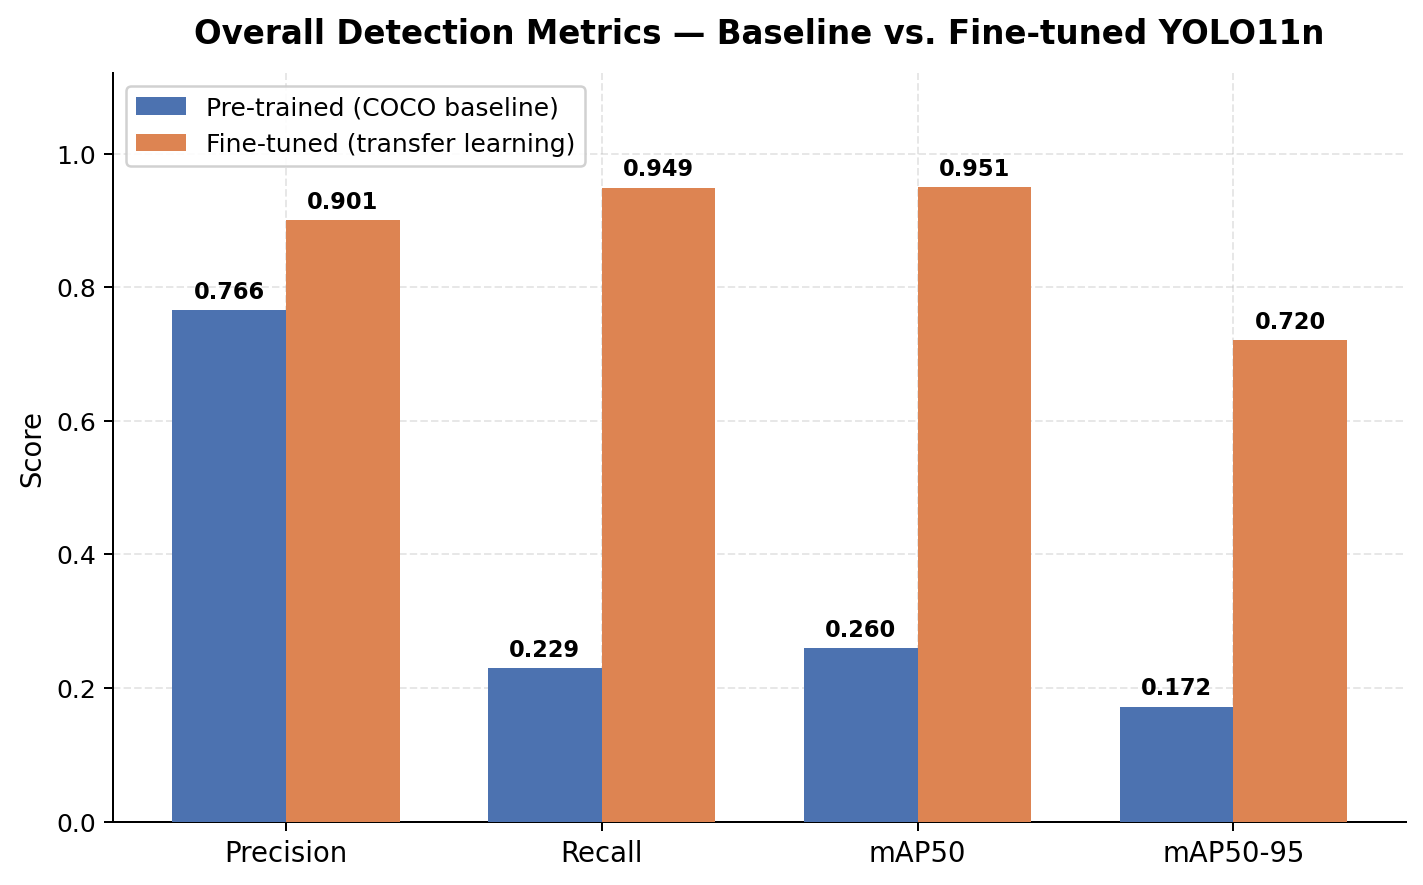
\includegraphics[width=0.90\linewidth]{01_overall_comparison.png}
  \caption{Overall Precision, Recall, mAP50, and mAP50-95 --- baseline (left bar)
           vs.\ fine-tuned (right bar) for each metric.}
\end{figure}

\begin{figure}[H]
  \centering
  \begin{subfigure}[b]{0.48\linewidth}
    \centering
    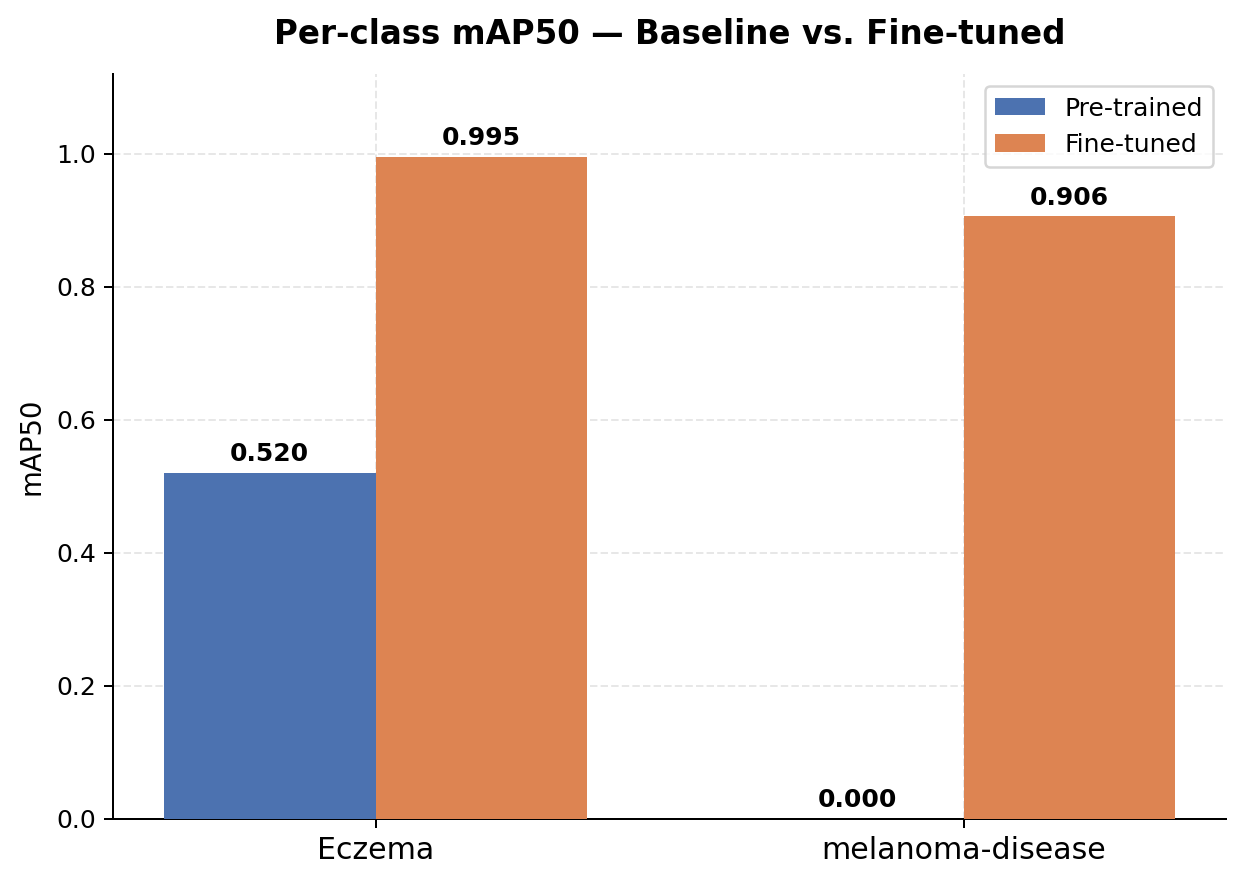
\includegraphics[width=\linewidth]{02_perclass_mAP50.png}
    \caption{Per-class mAP50.}
  \end{subfigure}
  \hfill
  \begin{subfigure}[b]{0.48\linewidth}
    \centering
    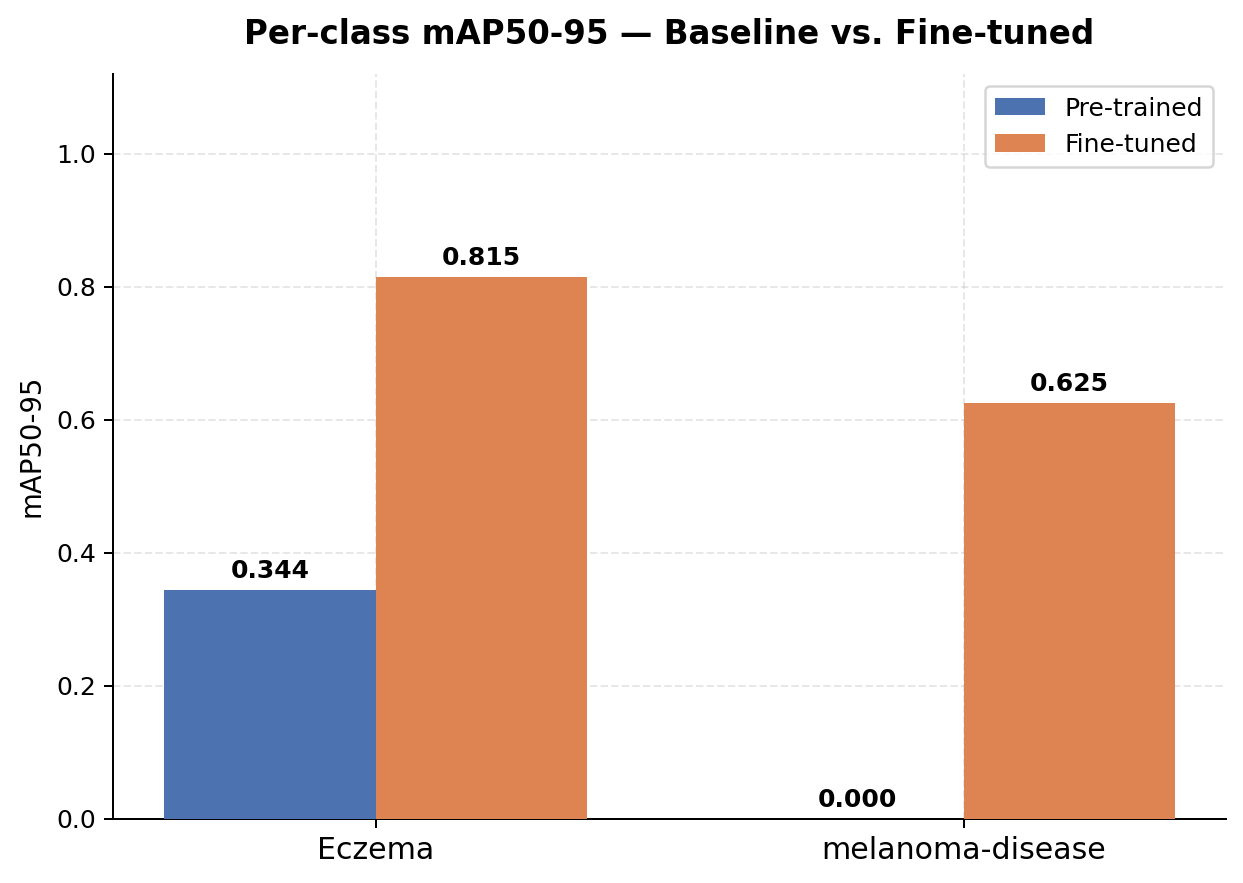
\includegraphics[width=\linewidth]{03_perclass_mAP50_95.png}
    \caption{Per-class mAP50-95.}
  \end{subfigure}
  \caption{Per-class mAP comparison. \texttt{melanoma-disease} improves from 0.000 to 0.906
           (mAP50) after fine-tuning.}
\end{figure}

\begin{figure}[H]
  \centering
  \begin{subfigure}[b]{0.44\linewidth}
    \centering
    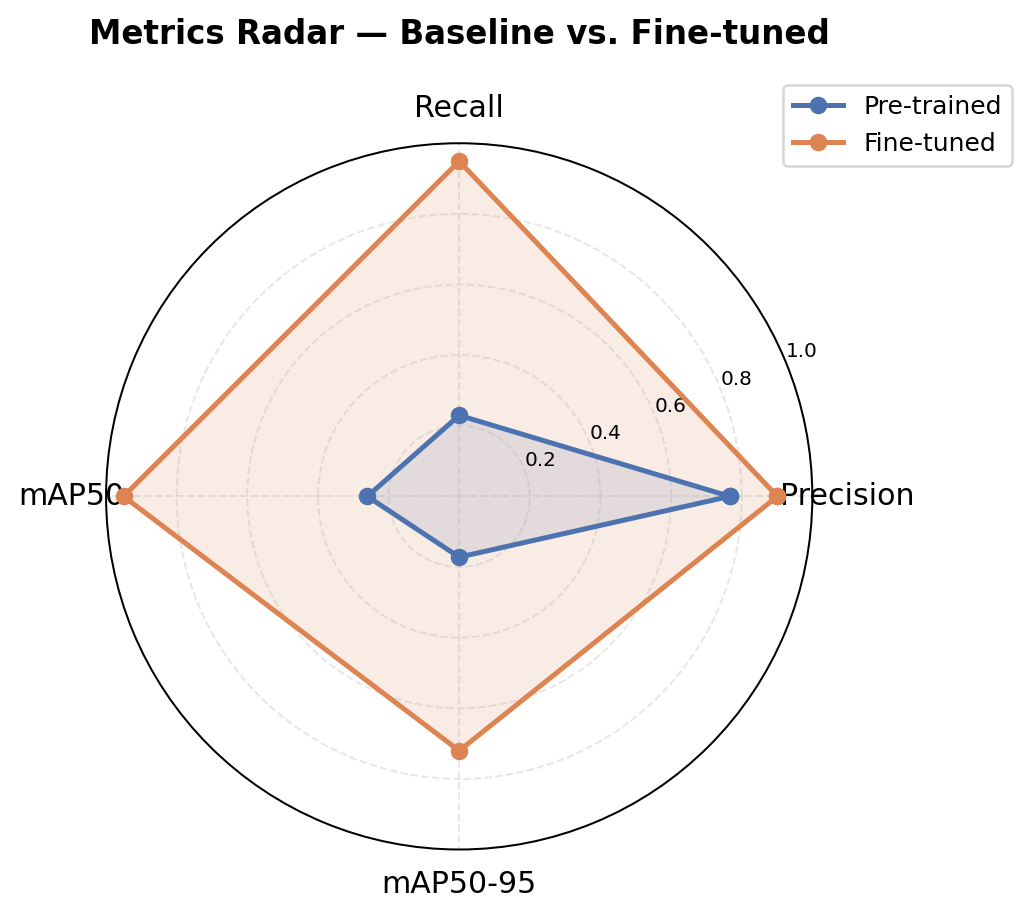
\includegraphics[width=\linewidth]{04_radar_chart.png}
    \caption{Radar chart of all four overall metrics.}
  \end{subfigure}
  \hfill
  \begin{subfigure}[b]{0.53\linewidth}
    \centering
    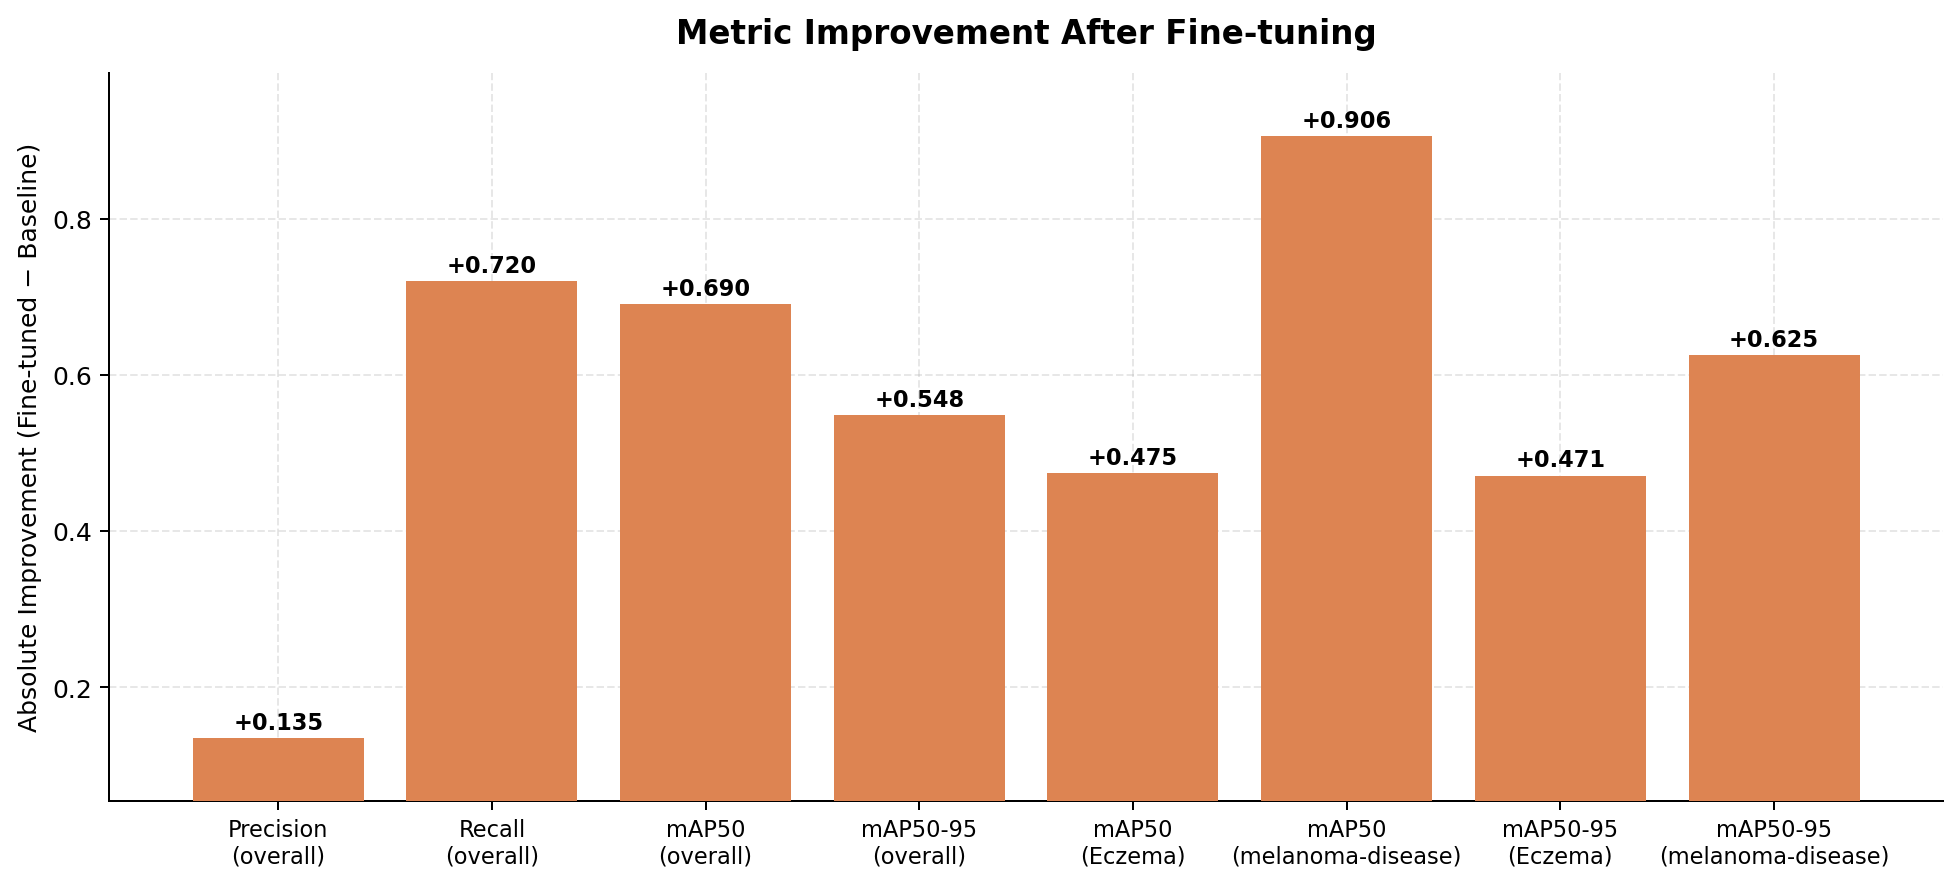
\includegraphics[width=\linewidth]{07_improvement_delta.png}
    \caption{Absolute improvement (fine-tuned $-$ baseline) per metric.}
  \end{subfigure}
  \caption{The fine-tuned model dominates the pre-trained baseline across every reported metric.}
\end{figure}

\begin{figure}[H]
  \centering
  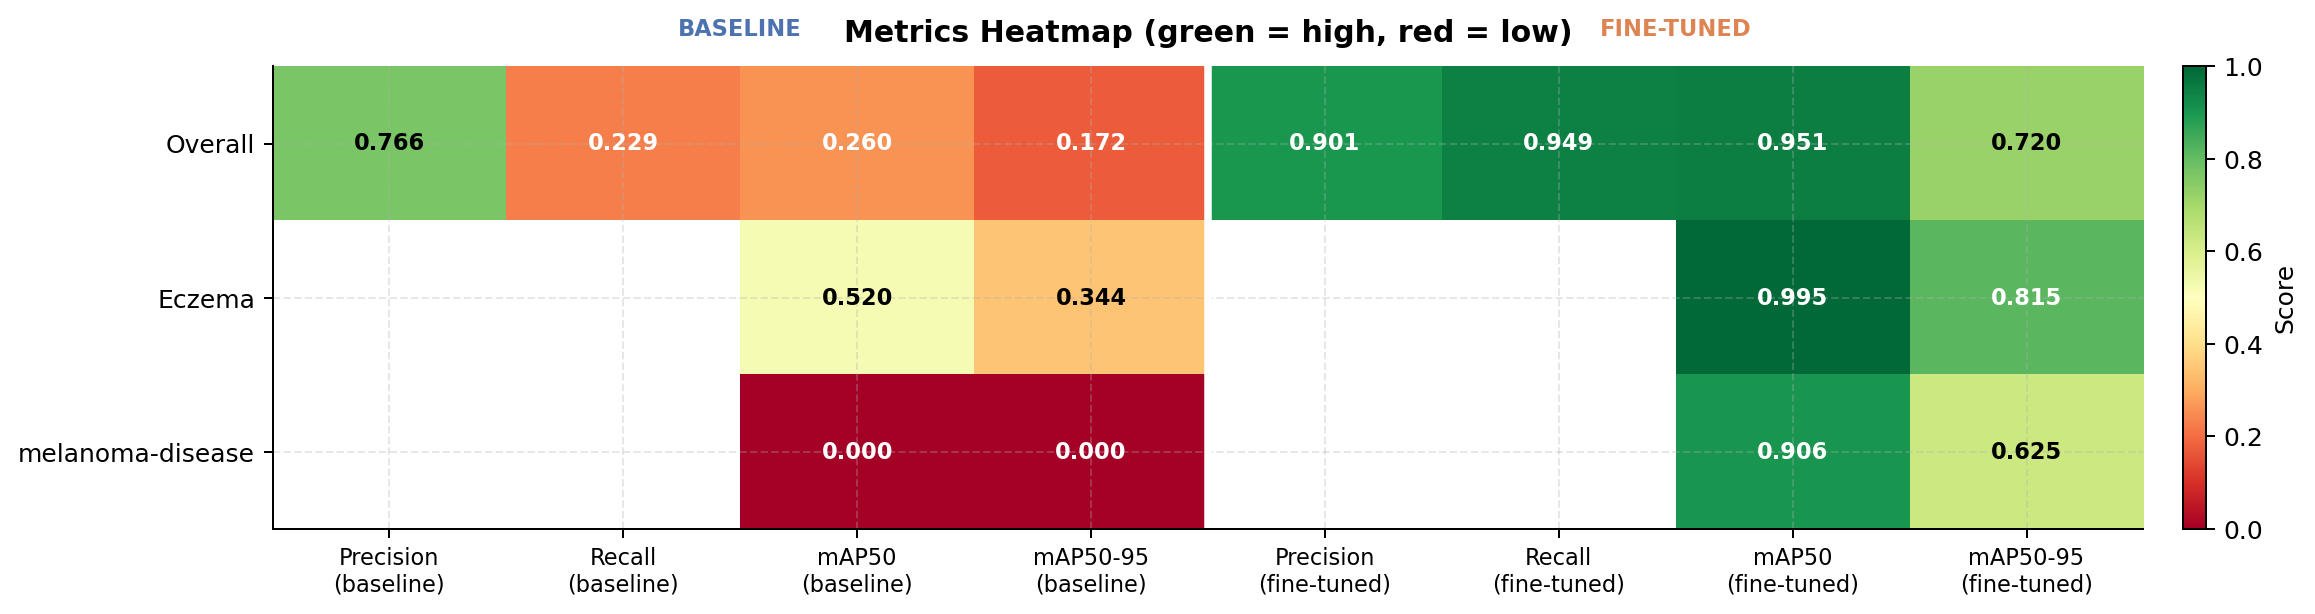
\includegraphics[width=\linewidth]{05_metrics_heatmap.png}
  \caption{Metrics heatmap (green = high score, red = low score). The fine-tuned columns are
           uniformly green; the baseline melanoma-disease cells are red (0.000).}
\end{figure}

% ── 5.2 Qualitative ─────────────────────────────────────────────────────────
\subsection{Qualitative Comparison}

\begin{figure}[H]
  \centering
  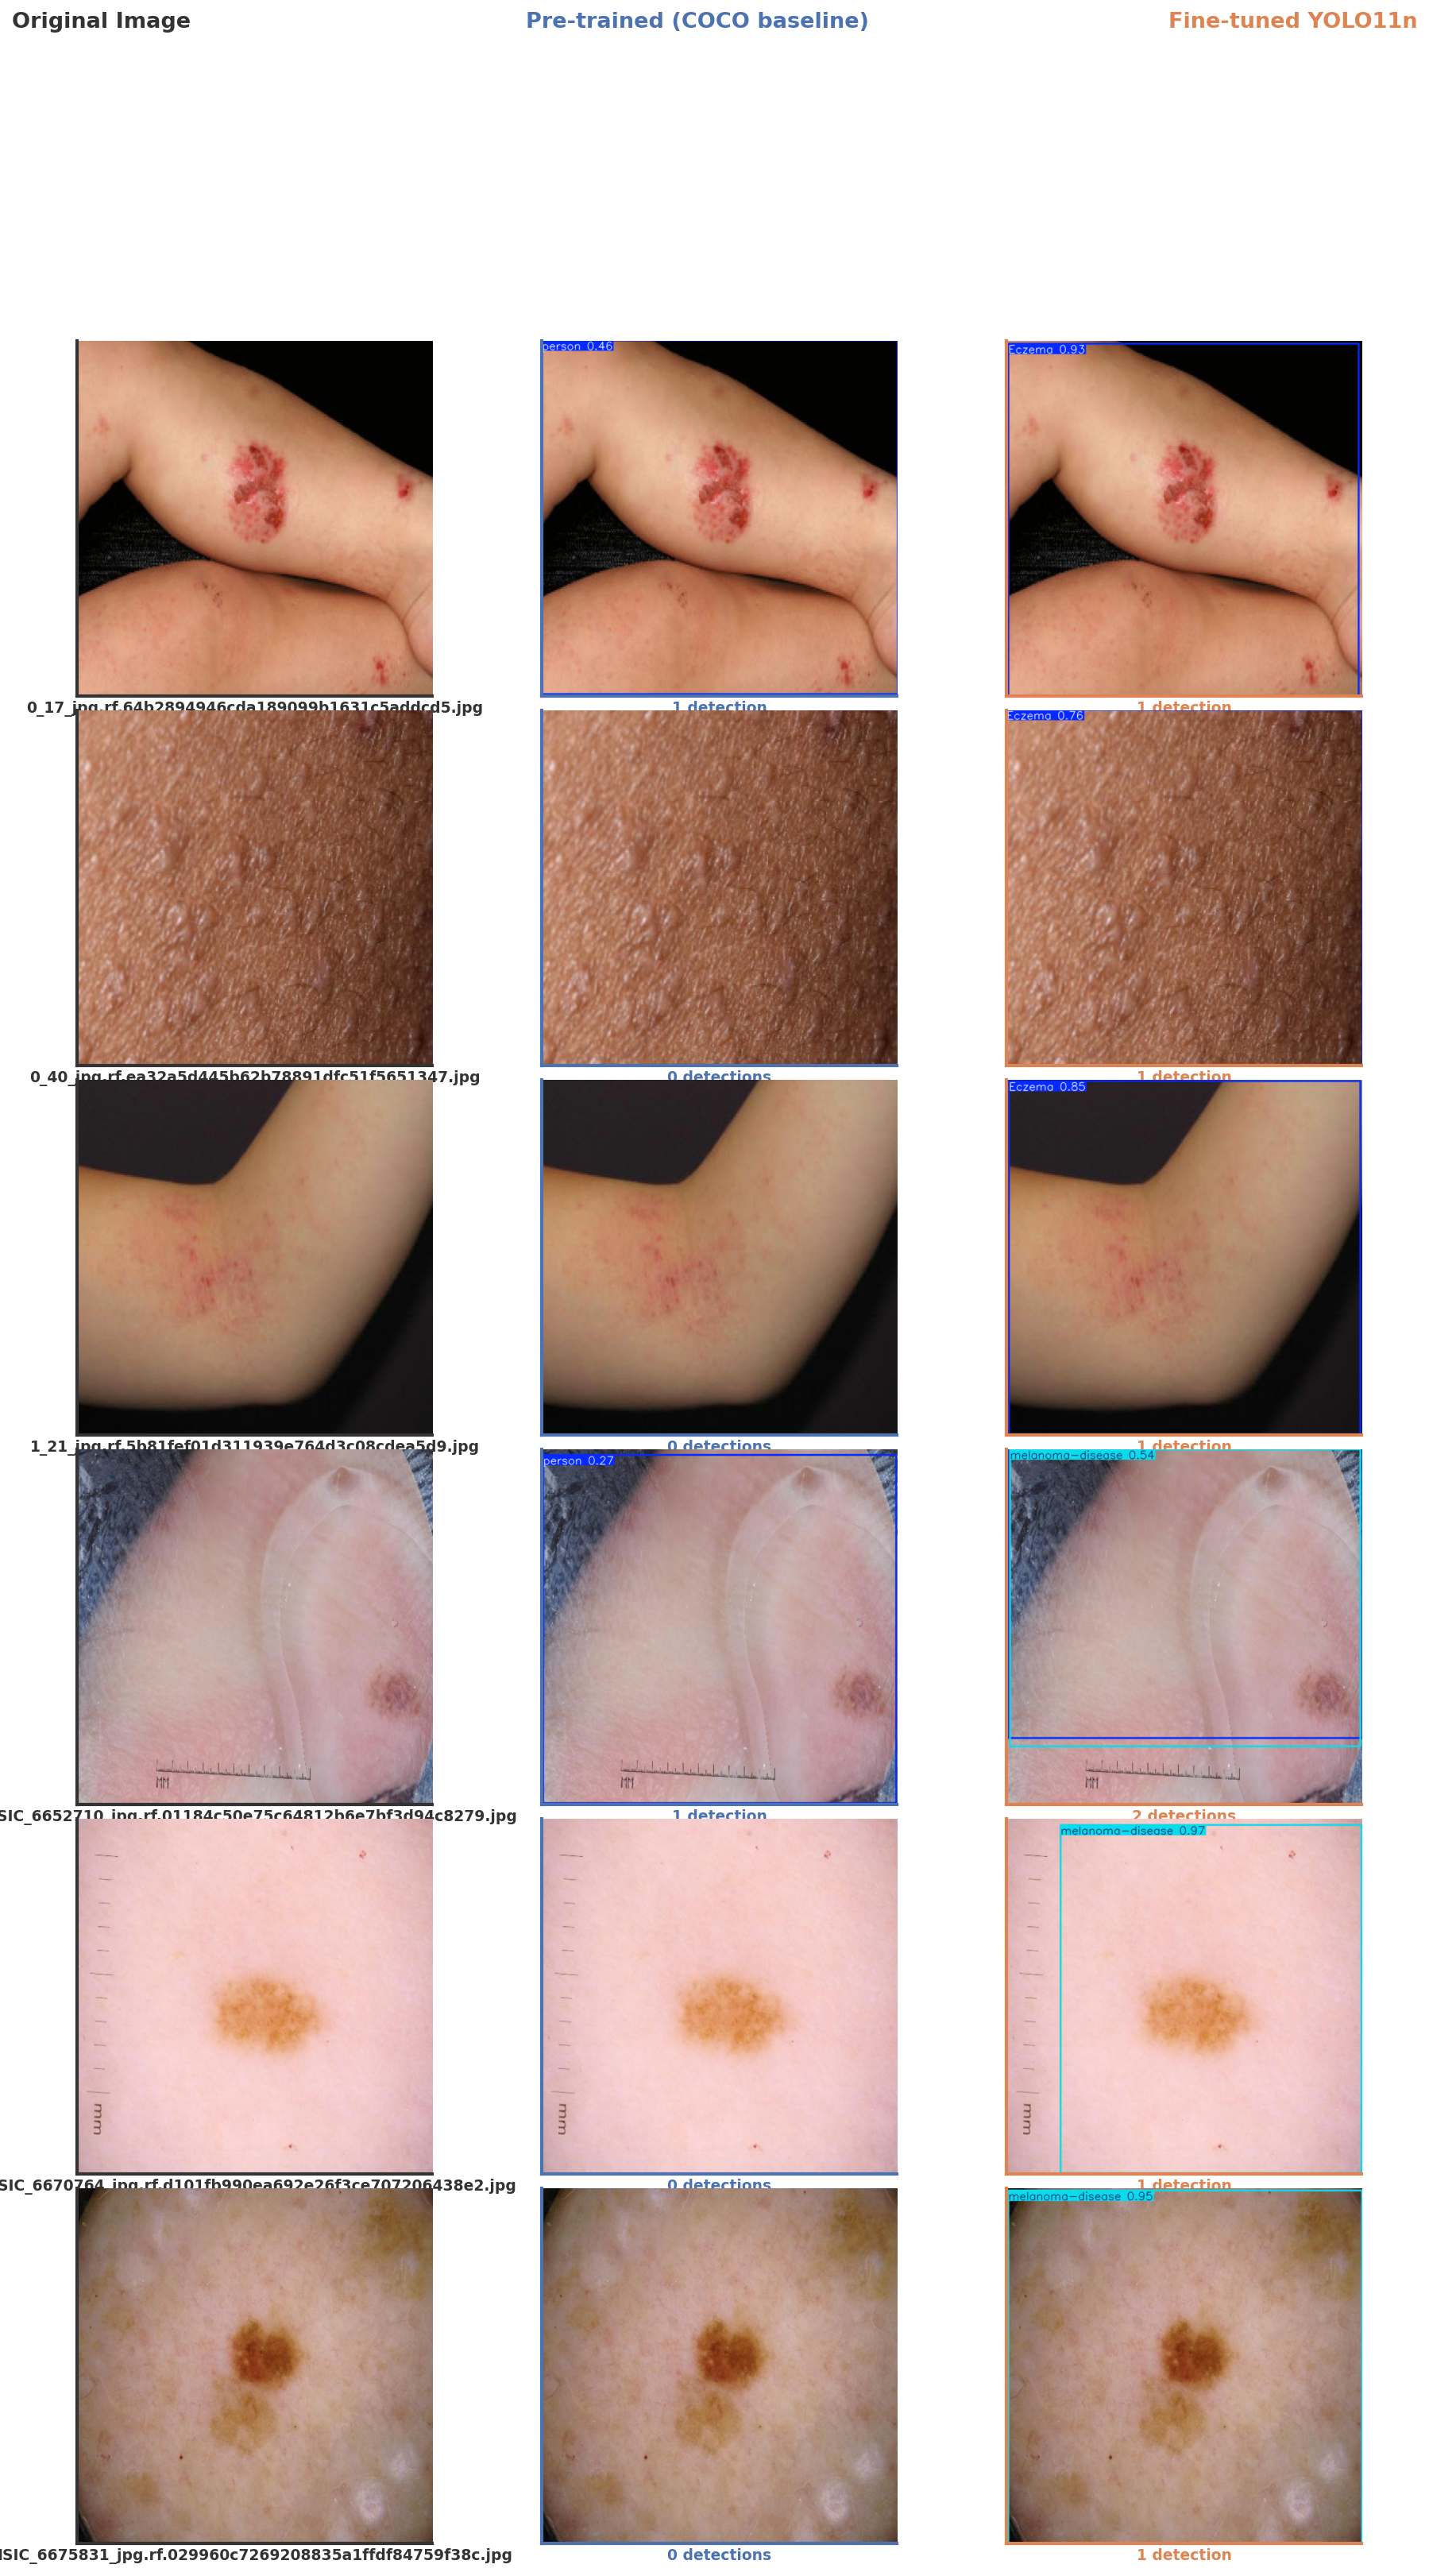
\includegraphics[width=\linewidth, height=0.88\textheight, keepaspectratio]{06_detection_comparison.png}
  \caption{Detection comparison on 6 test images. \textbf{Left:} original image.
           \textbf{Centre:} pre-trained (COCO) baseline --- mostly empty.
           \textbf{Right:} fine-tuned YOLO11n --- correct lesion detections with class labels
           and confidence scores.}
\end{figure}

\textbf{Discussion of improvement and remaining errors:}
\begin{itemize}[leftmargin=1.4em, itemsep=3pt]
  \item \textbf{melanoma-disease} goes from mAP50\,=\,0.000 (completely undetectable by the
        COCO model) to \textbf{0.906} --- demonstrating the necessity of transfer learning for
        domain-specific detection tasks.
  \item \textbf{Eczema} improves from 0.520 to \textbf{0.995}. The partial baseline score
        existed because the COCO model occasionally detected similar skin textures under generic
        classes (e.g.\ \emph{orange}, \emph{frisbee}).
  \item \textbf{Recall} jumps from 0.229\,$\to$\,0.949: the fine-tuned model finds nearly all
        lesions, whereas the baseline missed the vast majority.
  \item \textbf{Remaining errors:} occasional confusion between the two lesion types on images
        where Eczema and melanoma-disease share similar dermoscopic colouring and texture --- a
        known challenge in skin lesion analysis. A handful of false negatives persist on small
        lesions near image borders.
\end{itemize}

% ─────────────────────────────────────────────────────────────────────────────
\section{Gen-AI Reflection}

This project used \textbf{Claude} (claude-sonnet-4-6, Anthropic) throughout all stages:

\begin{itemize}[leftmargin=1.4em, itemsep=3pt]
  \item \textbf{Planning:} Claude designed the full five-step pipeline and selected the correct
        Roboflow dataset (discovering that the initially chosen dataset had only one class, then
        switching to \texttt{skin-k1hhx} with two classes).
  \item \textbf{Code generation:} All Python scripts and the Jupyter notebook were scaffolded
        by Claude and executed end-to-end. Scripts: \texttt{download\_dataset},
        \texttt{infer\_baseline}, \texttt{train\_finetune}, \texttt{evaluate}, \texttt{utils},
        \texttt{plot\_results}.
  \item \textbf{Report:} This \LaTeX{} report was drafted by Claude using actual training
        output, metrics, and generated figures.
  \item \textbf{Verification:} All generated code was executed and outputs (metrics,
        visualisations) were reviewed against expected behaviour. One bug was corrected during
        the run (absolute path rewriting in \texttt{data.yaml}).
\end{itemize}

\noindent\textbf{Tools used:} Claude (claude.ai/code), Roboflow SDK, Ultralytics YOLO Python
API, Tectonic (LaTeX engine), Matplotlib.

\vspace{12pt}
\noindent\rule{\linewidth}{0.4pt}
\vspace{2pt}
\begin{center}
  \small\textcolor{darkgray}{Submitted to Moodle --- May 2026 \quad|\quad
  Source code:
  \href{https://github.com/stellasdeutsch-dev/IVADL-Assignment-2}{github.com/stellasdeutsch-dev/IVADL-Assignment-2}}
\end{center}

\end{document}
